\chapter{FIDASIM: A Neutral Beam and Fast-ion Diagnostic Modeling Suite}\label{chap:fidasim}
In applying the forward models discussed in the previous chapter, one discovers that the process is more involved than simply evaluating the equations in the correct order. For instance, the forward models require a fast-ion distribution function, which is obvious; however, the form of the distribution function dictates the approach taken, e.g. the numerical approach for calculating the diagnostic signal generated by fast-ion distribution \textit{function} is very different from the approach taken when using a Monte Carlo distribution. Additionally, the diagnostic's forward model requires inputs that also need to be calculated, e.g. the neutral beam densities. The design of a diagnostic simulation system that is accurate, flexible, and computationally efficient was undertaken to address all the niggling implementation details. FIDASIM is the result. FIDASIM is a modern Fortran code that handles all the complexities inherent in applying the forward models outside of the ivory towers in which they were developed.  

\section{Brief History}
The development curve of FIDASIM is long and ongoing. 
The very first implementation of FIDASIM was written by Yadong Luo and Bill Heidbrink in IDL while Yadong was working on his thesis\cite{luo2007thesis}. Subsequently, Deyong Liu added features to simulate NPA signals. The IDL version of the code was distributed for public use and documented in a journal publication\cite{heidbrink2011code}.

The IDL version of FIDASIM was prohibitively slow---the average runtime for a single time slice was approximately 24 hours. As a part of his thesis\cite{geiger2013thesis}, Ben Geiger wrote the first version of FIDASIM written in Fortran 90. This prototype version was parallelized using OpenMP and was orders of magnitude faster, but it was not as easy to use as the IDL version and was difficult to port to different devices.

The further development of FIDASIM since 2013 is documented in this chapter. The goals of the new development were four-fold: to increase fidelity, to increase performance, to increase usability, and to generalize to other fusion devices. In pursuit of these goals, FIDASIM has been completely overhauled, bearing little resemblance to the version written by Ben Geiger. The current version of FIDASIM does the following: supports OpenMP and MPI parallelization, uses a faster FIDA and NPA algorithm, handles multiple types of fast-ion distributions, simulates neutrons and passive signals, uses HDF5 files over the previous custom binary files, is well documented, is used by multiple fusion devices, and more. In the following sections we will discuss the current design of FIDASIM. More information about FIDASIM can be found at the new documentation website: \url{http://d3denergetic.github.io/FIDASIM/}.

\section{User Inputs}
\subsection{Simulation Grids}
In physics simulations, the choice of simulation grid is a fork in the development roadmap. After a choice is made, the types of problems the code can solve is limited. Shakespeare once said, “The sins of the father are to be laid upon the children.”. A poor original design choice tends to haunt the development until it is eventually rectified via an exorcism. For instance, for many fusion codes it is common to tightly integrate the simulation grid with the magnetic equilibrium in the form of a field aligned coordinate system. This choice has several advantages; however, since the field aligned coordinate system is ill-defined outside the separatrix, the codes are limited to simulating phenomena that are within the separatrix. Attempts to rectify this original sin are cumbersome and complicated. At some point it is easier to just start over. 
This problem cannot be completely avoided, but it can be mitigated by careful design. When beginning development of a code, both the present and future use cases must be considered. A good design is able to grow with the increased scope of the code.

FIDASIM used two different simulation grids: the neutral beam grid, which holds the neutral beam densities and the interpolation grid, where all the plasma parameters and electromagnetic fields are defined.
\subsubsection{Neutral Beam Grid}
The neutral beam grid is an artifact from the original version of FIDASIM. In addition to its primary purpose of storing the results of the neutral beam, direct charge exchange (DCX), and thermal halo calculation, it was also the grid in which the electromagnetic fields, plasma parameters, and fast-ion distribution were defined. This design choice eventually became a problem and had to be removed. In the current version of FIDASIM, the neutral beam grid is relegated to storage duty although, like much of the code, it has been enhanced.

The neutral beam grid is a simple Cartesian grid where each of the three dimension is defined by a minimum/maximum value and the number of elements. In Ben Geiger's version of FIDASIM, that was the extent of the neutral beam grid definition. However, it is often useful to arbitrarily orient the grid---usually to align the grid with the neutral beam geometry. The original IDL version of FIDASIM had this feature. In order to reimplement the feature, the neutral beam grid definition was extended to include an origin and three Tait-Bryan rotation angles: $\alpha$, $\beta$, and $\gamma$. This allows the user to arbitrarily orient the neutral beam grid.

Some readers may be unfamiliar with Tait-Bryan rotation angles, which are also known as yaw, pitch, and roll angles. The Tait-Bryan angles were chosen because they, once learned, are more intuitive than the Euler angles taught in introductory classical mechanics courses. Like Euler angles, Tait-Bryan angles have different rotation conventions. FIDASIM uses the most common $z-y'-x''$ convention where the $\alpha$ angle corresponds to rotation about the $z$ axis, the $\beta$ angle corresponds to rotation about the $y'$ axis, and the $\gamma$ angle corresponds to rotation about the $x''$ axis. This process is demonstrated in Figure \ref{fig:tait_bryan}.
\begin{figure}[h!]
    \centering
    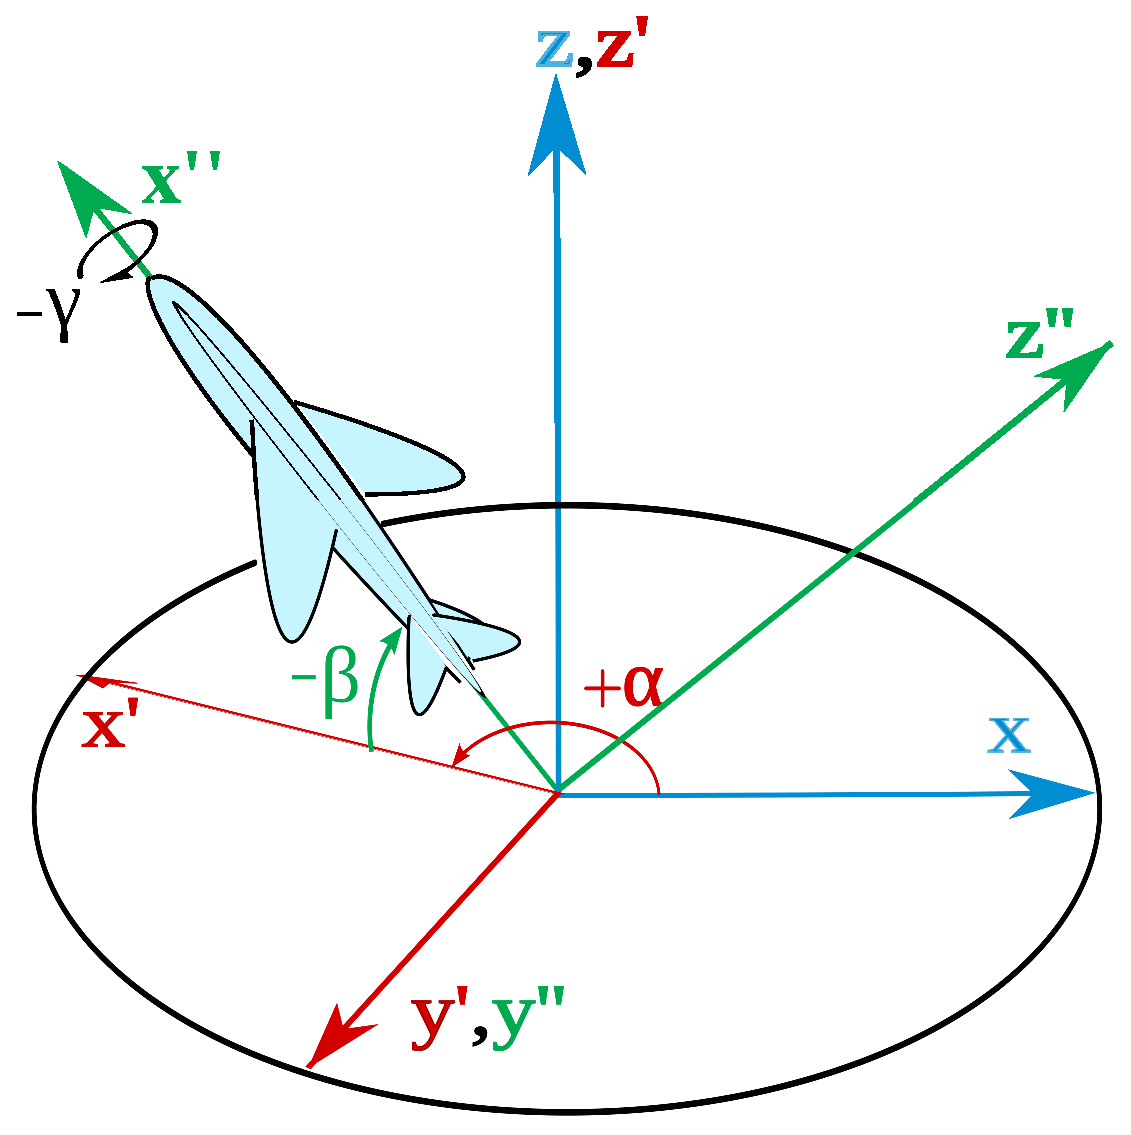
\includegraphics[width=8cm]{figures/tait_bryan.eps}
    \caption{$z-y'-x''$ rotation using Tait-Bryan angles. Figure modified from original image created by Wikipedia user Juansempere.}
    \label{fig:tait_bryan}
\end{figure}

The relationship between the unrotated machine coordinates and the rotated and shifted beam grid coordinates is given by
\begin{equation}\label{eq:xyz_to_uvw}
    \mathbf{uvw} = \mathbf{R}\cdot \mathbf{xyz} + \mathbf{origin}\,,
\end{equation}
where $\mathbf{R}$ is the rotation matrix defined by the Tait-Bryan angles, $\mathbf{uvw}$ and $\mathbf{xyz}$ are the position vectors in machine and beam grid coordinates, respectively. $\mathbf{origin}$ is the origin vector of the beam grid coordinates defined in machine coordinates.

The Tait-Bryan angles that align the beam grid with the neutral beam given two points along the beam centerline are given by
\begin{equation}
\begin{split}
    \alpha &= \arctan(v_2 - v_1,u_2 - u_1)
    \beta  &= \arcsin((w_1 - w_2)/D)
    \gamma &= 0
\end{split}
\end{equation}
with $D$ being the distance between the points.

\subsubsection{Interpolation Grid}
As mentioned, the electromagnetic fields, plasma parameters, and the fast-ion distribution function were originally mapped onto the neutral beam grid. This, however, created memory problems when the simulation domain was large or when fine spatial resolution was required. The main issue was with the mapping of the fast-ion distribution function. The mapped distribution was stored as a dense array with dimensions $(n_e,n_p,n_x,n_y,n_z)$. Increasing the number of neutral beam grid cells could very quickly outgrow the available memory. This situation was untenable as FIDASIM was starting to be used for the simulation of passive diagnostic signals from the cold edge neutrals, which fill up the entire vessel. In order to simulate the passive signals, the beam grid had to be expanded to cover a large volume. 

With the memory problems, resolution was sacrificed. To solve this problem, a 2D $R-Z$ grid was introduced. Instead of using an array look-up to determine the plasma parameters/fields within a beam grid cell, we would determine the parameters by interpolating on the 2D $R-Z$ grid. The interpolation grid solved the memory issues by exploiting the toroidal symmetry of a tokamak---more information with less space. However, with the switch to the interpolation grid we lost the ability to handle non-toroidally symmetric plasmas like stellarators. The option for 3D plasmas is currently being implemented into FIDASIM. This is being done by adding a toroidal $\phi$ variable to the interpolation grid definition. If the user does not provide $\phi$, then toroidal symmetry is assumed.

\subsection{Plasma Parameters}
In FIDASIM the plasma parameters are mapped to the interpolation grid. This is somewhat unusual. More commonly, the plasma parameters are represented as flux functions. This is usually a good choice; however, there are a few scenarios where a flux function is not the best choice. For example, in tokamak discharges with high torque the plasma tends to move out toward the wall, a consequence of the plasma's angular momentum. This can cause a mismatch in the plasma densities at the high and low field sides of a flux function. Additionally, the cold edge neutrals cannot be a flux function. There is also a matter of which flux label to support---$\psi$ or $\rho$---and how to deal with regions outside the separatrix. Mapping onto the interpolation grid was the most general choice that fixed the aforementioned issues.

FIDASIM takes in 2D profiles of the following plasma parameters: the electron density ($n_e\;\rm{cm^{-3}}$), the ion and electron temperature ($T_{i/e}\;\rm{keV}$), the plasma rotation ($\vec{v}\;\rm{cm/s}$) in cylindrical coordinates, the effective charge $Z_{eff}$, and the cold edge neutral density ($n_{cold}\;\rm{cm^{-3}}$). Within FIDASIM the impurity and ion densities are calculated from the user supplied inputs by manipulating the quasineutrality and $Z_{eff}$ formulas:
\begin{equation}
\begin{split}
    n_{imp} &= \frac{Z_{eff} - 1}{Z\,(Z-1)} n_e, \\
    n_i &= n_e - Z\,n_{imp}\,,
\end{split}
\end{equation}
where $Z$ is the charge number of the main impurity species.
\begin{figure}[h!]
    \centering
    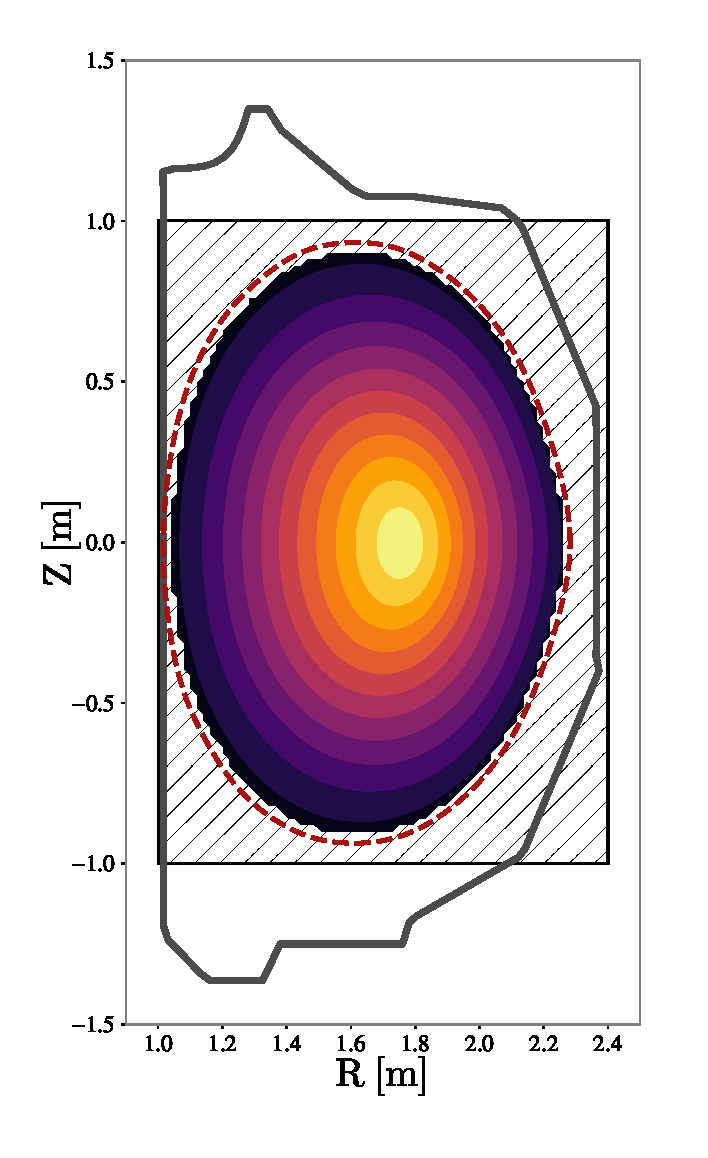
\includegraphics[width=8cm]{figures/te_cross_section.eps}
    \caption{Electron Temperature mapped onto the interpolation grid. Outside the separatrix (dashed red line) the plasma parameters are not set, i.e. the mask variable is set to 0.}
    \label{fig:te_mask}
\end{figure}
One complication that arises by not using flux functions is knowing when particles are outside the region where the plasma parameters are defined. FIDASIM uses a Boolean mask to indicate these regions. If the plasma parameters are defined at a given (R,Z), then the mask is one, otherwise, it is set to zero. Figure \ref{fig:te_mask} demonstrates the masking. For this particular time-slice the profiles were only provided up to the separatrix so the mask was set to one inside the separatrix and zero outside.

\subsection{Electromagnetic Fields}
In tokamaks the electromagnetic fields are determined by solving the Grad-Shafranov equation
\begin{equation}\label{eq:grad_shafranov}
    \Delta^* \psi = - \mu_0 R^2 \frac{dp}{d\psi} - \frac{1}{2}\frac{dg^2}{d\psi}\,,
\end{equation}
where $\Delta^*$ is the elliptic operator, $p(\psi)$ is the pressure, $g(\psi)$ is the poloidal current, and $\psi(R,Z)$ is the poloidal flux function.
The Grad-Shafranov equation is the equilibrium equation in ideal magnetohydrodynamics (MHD) for a two dimensional plasma. While FIDASIM does not solve this equation, electing to simply map the magnetic and electric fields in cylindrical coordinates onto the interpolation grid, it is useful to know how to extract the various fields from the poloidal flux so they can be used by FIDASIM.

The magnetic field, $\vec{B}$, in cylindrical coordinates is given by
\begin{equation}\label{eq:bfield}
\begin{split}
    B_R &=  \frac{1}{R}\frac{\partial \psi}{\partial Z}, \\
    B_Z &= -\frac{1}{R}\frac{\partial \psi}{\partial R}, \\
    B_{\phi} &= \frac{g(\psi)}{R}.
\end{split}
\end{equation}
The plasma current, $\vec{J}$, in cylindrical coordinates is given by
\begin{equation}\label{eq:jfield}
\begin{split}
    J_R &= -\frac{1}{\mu_0 R}\frac{\partial g}{\partial \psi} \frac{\partial \psi}{\partial Z}, \\
    J_Z &= \frac{1}{\mu_0 R}\frac{\partial g}{\partial \psi} \frac{\partial \psi}{\partial R}, \\
    J_{\phi} &= -R \frac{\partial p}{\partial \psi} - \frac{g(\psi)}{\mu_0 R}\frac{\partial g}{\partial \psi}.
\end{split}
\end{equation}
The plasma current is not used by FIDASIM; however, it is useful to know the sign of the dot product of the magnetic field and the plasma current, $\sigma = \rm{sign}(\vec{B}\cdot\vec{J})$, known as the pitch sign convention. This will become useful when we discuss the fast-ion distribution function.

To maintain force balance, a radial electric field, $E_r$, is induced. The electric field in cylindrical coordinates is given by
\begin{equation}\label{eq:efield}
\begin{split}
    E_R &= -R \frac{B_{pol}}{|\nabla \psi|} \frac{\partial \Phi}{\partial \psi} \frac{\partial \psi}{\partial R},\\
    E_Z &= -R \frac{B_{pol}}{|\nabla \psi|} \frac{\partial \Phi}{\partial \psi} \frac{\partial \psi}{\partial Z},\\
    E_{\phi} &= 0,
\end{split}
\end{equation}
where $\Phi(\psi)$ is the electric potential, and the poloidal magnetic field is given by $B_{pol} = \sqrt{B_R^2 + B_Z^2}$.


\subsection{Fast-ion Distribution}
Simulating the signals generated by a theoretical fast-ion distribution is FIDASIM's \textit{raison d'\^etre}, its reason for being. It is therefore important that FIDASIM is able to support multiple types of distributions.
Internally, FIDASIM can represent fast-ions using two different 6D coordinate systems. The most commonly used is the guiding center coordinates: the kinetic energy, $E$, the pitch of the fast ion with respect to the magnetic field, $p$\footnote{There are two different definitions of pitch that are used: pitch with respect to the magnetic field, $p = \vec{v}\cdot\vec{B}/(||\vec{v}||\,||\vec{B}||)$, and pitch with respect to the plasma current, $p = \vec{v}\cdot\vec{J}/(||\vec{v}||\,||\vec{J}||)$. To convert between the two conventions one only needs to multiply the pitch with the pitch sign convention, $\sigma$, discussed previously.}, the major radius, $R$, the elevation, $Z$, and the gyro and toroidal angles $\gamma$ and $\phi$. Less frequently used is the cylindrical coordinate system: $v_r$, $v_z$, $v_\phi$, $R$, $Z$, and $\phi$.
The coordinate system that FIDASIM uses depends on the type of the distribution that was supplied by the user; of which there are two(formerly one): guiding-center distribution functions, $F(E,p,R,Z)$, and Monte Carlo particle distributions.

\subsubsection{Guiding-center Fast-ion Distribution Function}
Like the plasma parameters, the fast-ion distribution function is mapped onto the interpolation grid (Fig. \ref{fig:fast_ion_distribution}). 
\begin{figure}
    \centering
    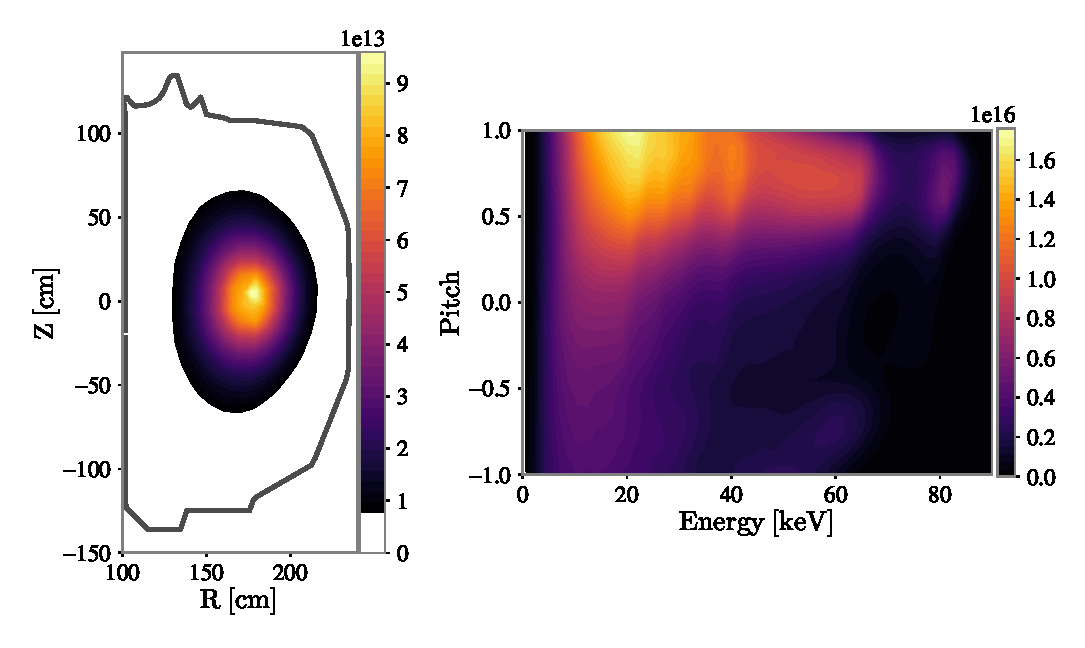
\includegraphics[width=13cm]{figures/fast_ion_distribution.eps}
    \caption{Projections of the guiding-center fast-ion distribution function for DIII-D discharge \#171469 at 1360 ms. Left: Velocity-space integrated fast-ion density. Right: Spatially integrated fast-ion velocity-space distribution. Pitch is defined relative to the plasma current.}
    \label{fig:fast_ion_distribution}
\end{figure}
It is assumed that the distribution is toroidally symmetric and the gyro-angle is distributed uniformly, $\gamma \sim \mathcal{U}(0,2\pi)$.
In this form, the total number of fast-ions is given by
\begin{equation}\label{eq:f_ntot}
    N_{f} = 2\pi \iiiint F(E,p,R,Z) R\,dE\,dp\,dR\,dZ.
\end{equation}
The integration over the gyro-angle is included in the definition of $F$.

\subsubsection{Monte Carlo Distributions}
A Monte Carlo distribution is defined by a set of $N_p$ Monte Carlo (MC) particles each with a set of attributes according to the coordinate system used. Guiding-center MC particles have a kinetic energy, pitch, R, Z, and weight ($w$). The full-orbit MC particles have a velocity in cylindrical coordinates, $\vec{v} = [v_r,v_z,v_\phi]$, R, Z, and weight.
For both types of MC distributions toroidal symmetry is assumed. For guiding-center MC distributions, it is assumed that the gyro-angle is distributed uniformly.
The weights of the particles are chosen such that the total number of fast ions is given by
\begin{equation}\label{eq:mc_ntot}
    N_{f} = \sum_i^{N_{p}} w_i \,.
\end{equation}
Since the particle weights include an implicit integration over the entire toroidal range, $[0,2\pi)$, for certain diagnostics, the weights are scaled by $\Delta \phi/2\pi$ where $\Delta \phi$ is the toroidal range of the simulation determined by the intersection of the MC particle with the neutral beam grid. This is done so $\phi$ can be efficiently sampled in a region where it is possible for signal to be produced, i.e. where there are neutrals with which to charge exchange.

\subsection{Atomic Tables}
As a neutral particle travels through a plasma, it undergoes several different types of interactions
\begin{itemize}
    \item charge exchange with Hydrogen and impurities
    \item excitation with electrons, Hydrogen, and impurities
    \item ionization with electrons, Hydrogen, and impurities
\end{itemize}
These cross sections, as well as Maxwellian averaged reaction rates, are pre-computed over a range of logarithmically spaced collision energies and target temperatures. The sources of all the cross sections are given in Appendix \ref{app:cross_sections}. 
However, some of the atomic transitions needed by FIDASIM are not available. In particular, FIDASIM needs the n/m-resolved charge exchange cross sections. While certain transitions are available through ADAS\cite{adas} and other sources, others are not, as such, certain approximations are needed to fill out the table.

For instance, we use the equivalence principle (reversibility formula) to mirror the known ADAS cross sections.
\begin{equation}\label{eq:equilvalence}
    \sigma(n_f \rightarrow n_i) = \frac{E_i}{E_f}\frac{n_i^2}{n_f^2}\sigma(n_i \rightarrow n_f)
\end{equation}
However, this is insufficient to completely fill out the needed transitions.
Fortunately, since the \textit{total} cross sections for a transition $n \rightarrow m$ are given by Janev\cite{janev2003collision}, we can make the assumption that the probability of a transition decreases exponentially with the difference in energy between the levels. So long as we make sure the total cross section remains unchanged, we can "spread" the total cross section among the different unknown transitions.
A summary of the various approximations used in the charge exchange tables is given in Table \ref{tab:cx_sources}.
\begin{table}[ht]
\centering
\caption{Charge exchange cross section sources. Total cross sections for $n>4$ are not available so the $n=4$ total cross sections are used. The $m$ levels are normalized to the Janev\cite{janev2003collision} tables for consistency. Spreading is done over the $m$ values/rows}
\label{tab:cx_sources}
\resizebox{\textwidth}{!}{\begin{tabular}{c|c|c|c|c|c|c|c}
\textbf{n/m}        & \textbf{1}                          & \textbf{2}                          & \textbf{3}                          & \textbf{4}                    & \textbf{5}                    & \textbf{6}                    & \textbf{Total}  \\ \hline
\textbf{1} & {\color[HTML]{CB0000} ADAS}         & {\color[HTML]{CB0000} ADAS}         & {\color[HTML]{CB0000} ADAS}         & {\color[HTML]{CB0000} ADAS}   & {\color[HTML]{00009B} Spread} & {\color[HTML]{00009B} Spread} & Janev(n=1)      \\ \hline
\textbf{2} & {\color[HTML]{036400} Equivalence}  & {\color[HTML]{CB0000} ADAS}         & {\color[HTML]{CB0000} ADAS}         & {\color[HTML]{00009B} Spread} & {\color[HTML]{00009B} Spread} & {\color[HTML]{00009B} Spread} & Janev(n=2)      \\ \hline
\textbf{3} & {\color[HTML]{036400} Equivalence} & {\color[HTML]{CB0000} ADAS}         & {\color[HTML]{CB0000} ADAS}         & {\color[HTML]{CB0000} ADAS}   & {\color[HTML]{CB0000} ADAS}   & {\color[HTML]{00009B} Spread} & ADAS/Janev(n=3) \\ \hline
\textbf{4} & {\color[HTML]{036400} Equivalence} & {\color[HTML]{036400} Equivalence} & {\color[HTML]{036400} Equivalence} & {\color[HTML]{00009B} Spread} & {\color[HTML]{00009B} Spread} & {\color[HTML]{00009B} Spread} & Janev(n=4)      \\ \hline
\textbf{5} & {\color[HTML]{00009B} Spread}       & {\color[HTML]{036400} Equivalence} & {\color[HTML]{036400} Equivalence} & {\color[HTML]{00009B} Spread} & {\color[HTML]{00009B} Spread} & {\color[HTML]{00009B} Spread} & Janev(n=4)      \\ \hline
\textbf{6} & {\color[HTML]{00009B} Spread}       & {\color[HTML]{036400} Equivalence} & {\color[HTML]{036400} Equivalence} & {\color[HTML]{00009B} Spread} & {\color[HTML]{00009B} Spread} & {\color[HTML]{00009B} Spread} & Janev(n=4)     
\end{tabular}}
\end{table}

In addition to the cross sections, we also need the beam-plasma reaction rates, which we can readily calculate from the cross sections. With the assumption that the fast-ion density is small compared to the thermal density (below \%20), the beam-plasma reaction rate is given by an average over a Maxwellian,
\begin{equation}\label{eq:full_reaction_rate}
    \langle \sigma v \rangle = \iint \sigma(E_{rel}) ||\mathbf{v} - \mathbf{v'}|| \delta(\mathbf{v'}-\mathbf{v}_B) \left [ \frac{m_T}{2\pi kT} \right ]^{\frac{3}{2}} e^{-\frac{m_T}{2kT}(\mathbf{v}\cdot\mathbf{v})} d\mathbf{v}'\,d\mathbf{v} ,
\end{equation}
where $\mathbf{v}_B$ is the beam velocity, $m_T$ is the mass of the plasma/target species, and $T$ is the plasma temperature. Calculating the reaction rate requires integrating over a range of velocities. This creates a slight inconvenience when tabulating the rates since the spread of velocities would change depending on the temperature. To ameliorate this, a simplified form of Equation \ref{eq:full_reaction_rate} that uses normalized velocities, $u_{r/z}$, is used to calculate the reaction rates. The simplified reaction rate equation takes the form
\begin{equation}\label{eq:reaction_rate}
\langle \sigma v \rangle = \frac{2}{\sqrt{\pi}}\sqrt{\frac{2kT}{m_T}} \iint \sigma(E_{rel}) \sqrt{u_r^2 + \left (u_z - \sqrt{\frac{E_B m_T}{m_B kT}}\right)^2}  e^{-(u_r^2 + u_z^2)}u_r \,du_r\,du_z\,,
\end{equation}
where $m_B$ and $E_B$ is the mass and energy of the beam species respectively. In terms of the normalized velocities, the relative energy of collision, $E_{rel}$ is given by
\begin{equation}\label{eq:e_rel}
E_{rel} = \mu \frac{kT}{m_T} \left ( u_r^2 + \left(u_z - \sqrt{\frac{E_B m_T}{m_B kT}}\right)^2 \right )\,,
\end{equation}
where $\mu$ is the reduced mass of the species.
To find the reaction rate, Equation \ref{eq:reaction_rate} is integrated from a normalized velocity of $-4$ to $4$ in both the $r$ and $z$ directions.
The full derivation of the reaction rate equation is given in Appendix \ref{app:reaction_rate}. 

%===============================================================================
%===============================================================================
%===============================================================================
\section{Simulation of Neutral Populations}
The neutral densities are an important part of the fast-ion diagnostics forward models and require careful modeling.
There are four neutral populations that FIDASIM simulates: the neutral beam which consists of full, half, and third energy components, the thermal halo, fast neutrals, and the cold edge neutrals.
With the exception of the cold edge neutrals, the algorithm for simulating the different neutral populations are remarkably similar, differing only in their initial conditions and possible trajectories through the plasma.

\subsection{Neutral Particle Trajectories}
The amount of neutrals produced by a source is distributed among the particle trajectories produced by the source. The trajectories the neutral particles take is determined by the local neutral velocity distribution, which is taken to be the ion distribution for neutrals born of charge exchange. The number of trajectories used in the calculations, $N_t$, is a user input and is typically set to be very large ($\sim10^6$) to best represent the true distribution. The more trajectories used, the more accurate the result.

The neutral particles trajectory through the neutral beam grid is used prolifically within FIDASIM as the time spent in each cell is needed to solve the collisional radiative model (COLRAD)(Eq. \ref{eq:colrad}, \ref{eq:neutral_population}), which determines how the neutrals are distributed along the cells in the track. Summing the contributions of each trajectory determines the total spatial profile of the neutrals. The tracking through the beam grid could be done at the same time as COLRAD, but pre-computing the track allows us to be able to short-circuit certain calculations; avoiding the computationally expensive COLRAD calculation. For instance, in the FIDA calculation, if a fast neutral doesn't cross a line of sight, it can't contribute signal; therefore, there is no need for the full calculation.

The particle tracking algorithm is as follows.
Each 3D cell in a grid is defined by 6 surfaces. In the case of a Cartesian grid, the cell is defined by the intersection of 6 planes, for a cylindrical grid a cell is defined by 4 planes and 2 cylinders. Given an initial starting point and velocity, the time it takes to intersect each surface is calculated. The smallest non-negative time, $t_{min>0}$, is the time spent in the cell. Information about the cell is collected and the neutral particle's position is advanced by $t_{min>0}$. This process repeats until the neutral particle exits the grid.

\subsection{Beam Neutrals}
The geometry of a neutral beam is defined by a source position and an axis such that a point along the beam centerline is defined as
\begin{equation}\label{eq:nbi_geom}
    \vec{C}(t) = \vec{s} + \vec{a} \cdot t\,,
\end{equation}
where $\vec{C}(t)$ is the position along the beam centerline parameterized by $t$, $\vec{s}$ is the source position, and $\vec{a}$ is the axis. The ion source is defined by its shape (circular or rectangular), size (half width and half height), vertical and horizontal focal lengths, and an energy dependent divergence. 

The trajectory of a beam neutral is determined by the following equations:
\begin{equation}\label{eq:beam_trajectory}
    \begin{split}
        v_x &= 1  \\
        v_y &= v_x\left(-\frac{y_s}{f_y} + \tan(\theta_y)\right),\quad \theta_y \sim \mathcal{N}(0,\beta_y^2) \,,\\
        y_z &= v_x\left(-\frac{z_s}{f_z} + \tan(\theta_z)\right),\quad \theta_z \sim \mathcal{N}(0,\beta_z^2)\,,
    \end{split}
\end{equation}
where $v_x$ points towards the plasma, $y_s$ and $z_s$ are random positions on the source plate in the horizontal and vertical directions respectively, $f_{y/z}$ are the focal lengths, and $\beta_{y/z}$ are the divergences. Examples of the different trajectories generated by the above equations are shown in Figure \ref{fig:beam_divergence}.
\begin{figure}[ht]
    \centering
    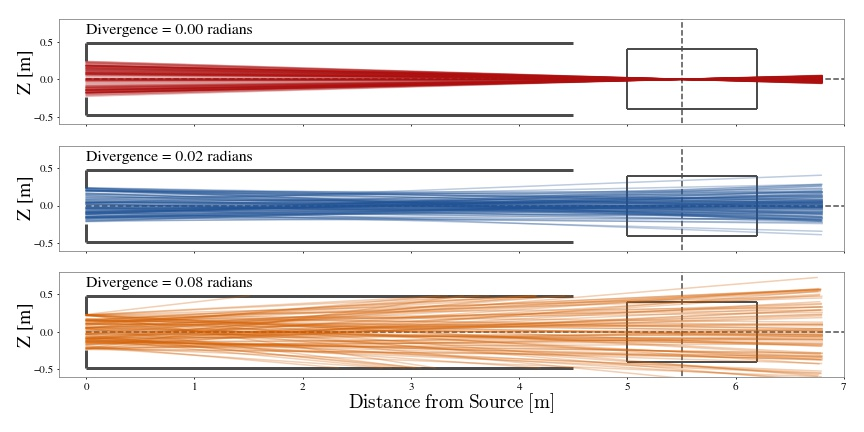
\includegraphics[width=15cm]{figures/beam_divergence.jpg}
    \caption{The effects of different beam divergences on beam particle trajectories. Focal length (dashed vertical line) is fixed at 5.5 m.}
    \label{fig:beam_divergence}
\end{figure}
Not shown in the above figure are the beam aperture(s), which collimate the neutral beam. Apertures are represented in FIDASIM by their shape (circular or rectangular), size (half width and half height), offsets relative to the +x aligned beam centerline, and their distance from the source grid. It is assumed that the plane of the aperture(s) is parallel to the plane of the source grid.

With the neutral beam geometry, we are able to approximate the beam neutral velocity distribution at a given point. The beam neutral velocity distribution, $f_b$, in beam grid coordinates is proportional to
\begin{equation}\label{eq:beam_distribution}
    f_b(\vec{v}) \propto \frac{\cos^2(\theta_y)\cos^2(\theta_z)}{2\beta_y\beta_z}\exp\left(-\left(\frac{\theta_y^2}{2\beta_y^2} + \frac{\theta_z^2}{2\beta_z^2}\right)\right)I(\vec{v},y_s,z_s)\,,
\end{equation}
where $I(\vec{v},y_s,z_s)$ is a function that indicates that the trajectory is possible and the angles $\theta_{y/z}$ are found via Equation \ref{eq:beam_trajectory}. Normalization aside, in vacuum, the above equation is exact; however, attenuation within the plasma weights each possible trajectory differently, incurring a slight error. Although not done in FIDASIM, appending a trajectory dependent attenuation factor to Equation \ref{eq:beam_distribution} would correct for it.\footnote{It should be noted that Equation \ref{eq:beam_distribution} is only used in FIDASIM for the calculation of approximate spectra. In the full calculation, attenuation is properly accounted for.}

During the acceleration phase of neutral beam injection, multiple atomic and molecular species are accelerated to the same kinetic energy,$E_{inj}$. During the neutralization phase, the molecular species are split apart, creating neutral populations with different energies: $E_{inj}$, $E_{inj}/2$, and $E_{inj}/3$. These different beam populations are called the Full, Half, and Third energy components, respectively.
Each beam component attenuates differently in the plasma and needs to be treated separately.
\begin{figure}[h!]
    \centering
    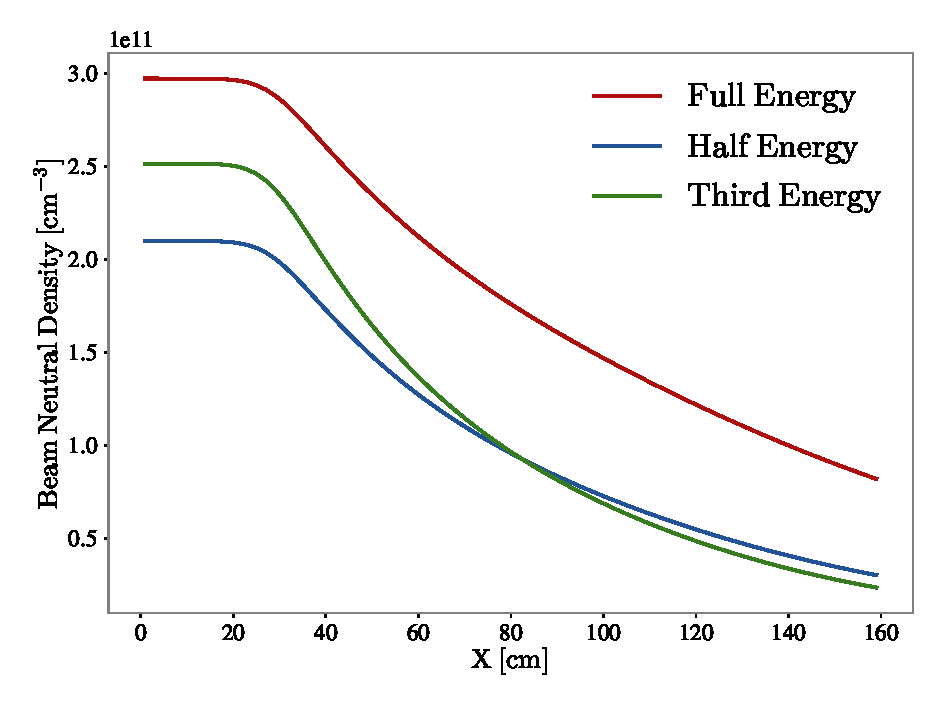
\includegraphics[width=10cm]{figures/beam_attenuation.eps}
    \caption{Attenuation of the different beam species for a DIII-D discharge. Density is summed over the y and z directions.}
    \label{fig:beam_attenuation}
\end{figure}
For a single beam trajectory, it is assumed that the beam neutral for the i$_{th}$ energy component is in the ground ($n=1$) state with initial population flux given by
\begin{equation}\label{eq:nb_flux}
    f_1(t=0)|_i = \left. \frac{d n_1}{dt}\right\rvert_i = \frac{C_i}{N_t} \cdot \frac{d n_{tot}}{dt}\,,
\end{equation}
where $C_i$ is the components current fraction, $N_t$ is the number of beam trajectories, and $dn_{tot}/dt$ is the total population flux of neutrals given by
\begin{equation}\label{eq:tot_flux}
    \frac{d n_{tot}}{dt} = \frac{P_{inj}}{\sum_i^3 C_i E_{inj}/i}\,,
\end{equation}
where the numerator, $P_{inj}$, is the total beam power and the denominator is the average beam energy.
The current fractions are a measured quantity that are specific to a neutral beam. For DIII-D's neutral beams, the current fractions are a function of the injection energy and are given by
\begin{equation}\label{eq:d3d_cfracs}
\begin{split}
    C_{1}(E_{inj}) &= -0.109171 + 0.0144685\, E_{inj} - 7.83224\times10^{-5}\, E_{inj}^2 \\
    C_{2}(E_{inj}) &= 0.0841037 + 0.0025516\, E_{inj} - 7.42683\times10^{-8}\, E_{inj}^2 \\
    C_{3}(E_{inj}) &= 1 - C_{1} - C_{2}
\end{split}
\end{equation}

As the neutral travels through the grid, it will be attenuated by the plasma and neutrals will be deposited in each cell it crosses. Figure \ref{fig:beam_attenuation} shows the attenuation of the different beam species as they travel through the plasma. To get the total beam density, the above process is repeated for the $N_t$ beam trajectories and the results summed. Figure \ref{fig:beam_density}a shows the neutral beam profile.
\begin{figure}[h!]
    \centering
    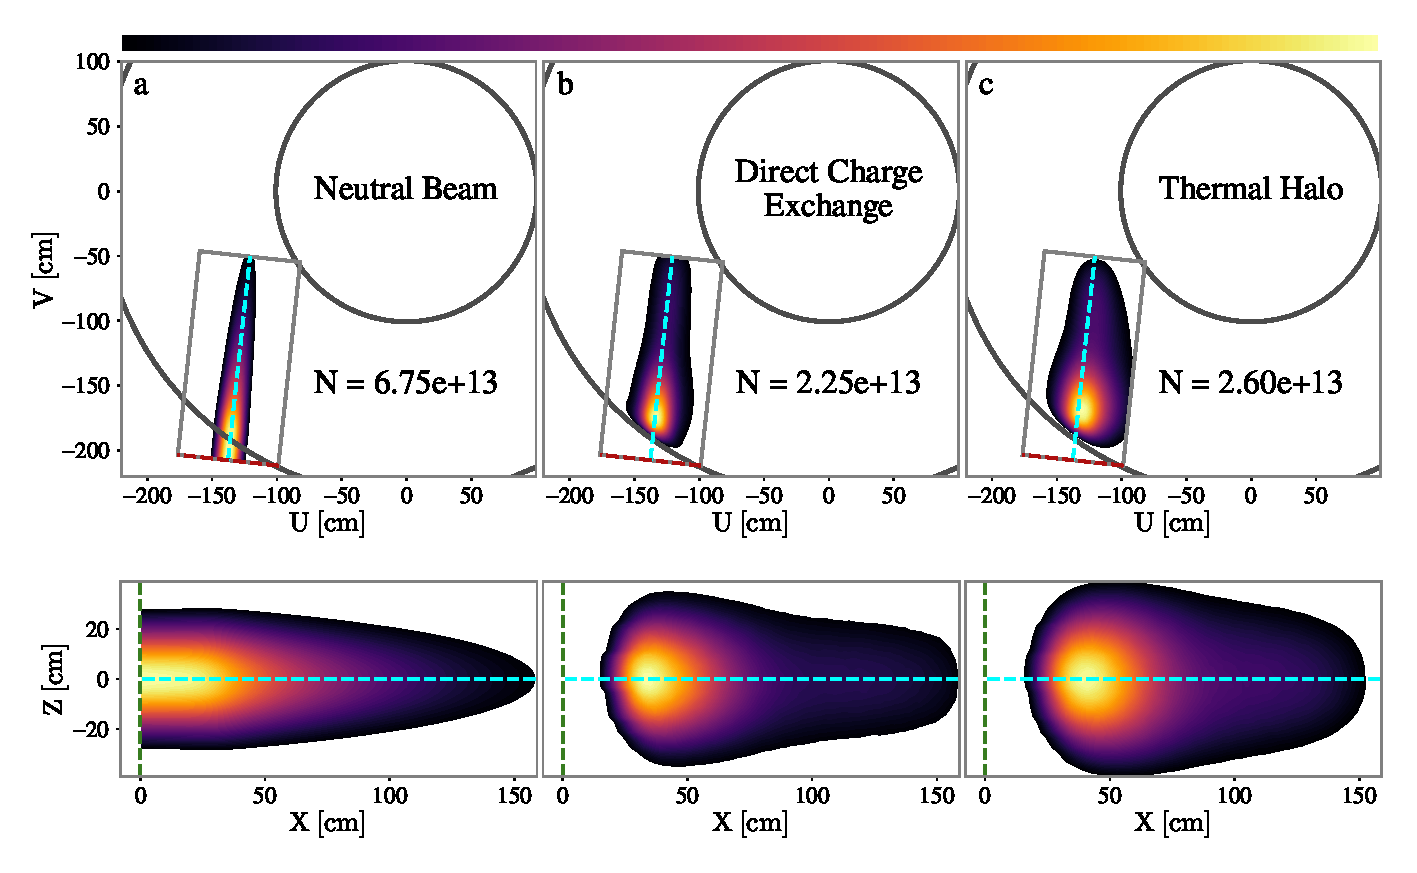
\includegraphics[width=16cm]{figures/beam_density.eps}
    \caption{Neutral profiles for the neutral beam (Column a), direct charge exchange (DCX) (Column b), and thermal halo (Column c). Top row: 2D profiles in machine coordinates, integrated over $W$. Bottom row: 2D profiles in beam grid coordinates, integrated over $Y$. The beam grid axes are color coded: $X$ axis (dashed cyan), $Y$ axis (dashed red), and $Z$ axis (dashed green) The number of neutrals in each population is listed. The colormap on top increases from left to right. The beam geometry is the 210RT neutral beam on DIII-D.}
    \label{fig:beam_density}
\end{figure}

\subsection{Direct Charge Exchange and Halo Neutrals}
Beam neutrals, $H_b$, can undergo charge exchange with thermal ions, $H_{th}^+$, creating a new neutral population. This population is called the direct charge exchange (DCX) neutrals. The initial population flux for a DCX neutral born in a cell with beam density, $\mathbf{d}_i$, is given by
\begin{equation} \label{eq:dcx_rates}
    \mathbf{f}(t=0) = \frac{N_{th}}{N_{t}}\sum_{i=1}^3 \left [ \int \mathbf{X}(\mathbf{v}_{DCX} - \mathbf{v}) \cdot \mathbf{d}_i\, ||\mathbf{v}_{DCX} - \mathbf{v}||\, f_i(\mathbf{v})\, d\mathbf{v} \right ]\,,
\end{equation}
where $\mathbf{X}$ $[cm^2]$ is a matrix of the charge exchange cross sections, $f_i$ is the velocity distribution of the $i^{th}$ beam energy component, $\mathbf{v}_{DCX}$ is the DCX neutral velocity, $N_{th}$ is the number of thermal ions in the cell, and $N_{t}$ is the number of trajectories the DCX neutral could take. The trajectories are determined from the local thermal ion velocity distribution that takes the form of a shifted Maxwellian.

After the initial population flux is determined, the DCX neutral travels ballistically and deposits neutrals along its trajectory in accordance with the collisional radiative model. The DCX density produced by a cell is determined by summing the contributions from each DCX trajectory. The total DCX density is calculated by repeating the above process for every cell that contains a beam neutral.

Likewise, the DCX neutrals can also undergo charge exchange with the thermal ions, creating a new neutral population that will then also undergo charge exchange with the thermal ions. The process of a neutral population charge-exchanging with the thermal ions can repeat ad infinitum; each new generation producing fewer neutrals than the generation before it. The overall effect is a thermal Halo of neutrals surrounding the neutral beam. The iterative process is demonstrated in Equation \ref{eq:dcx_halo_iteration}.
\begin{equation}\label{eq:dcx_halo_iteration}
\begin{split}
\rm{DCX\,\,:} \quad &H_{th_0}^+ + H_b \rightarrow H_{th_0} + H_b^+\\
\rm{Halo\,:} \quad &H_{th_1}^+ + H_{th_0} \rightarrow H_{th_1} + H_{th_0}^+\\
\rm{Halo\,:} \quad &H_{th_2}^+ + H_{th_1} \rightarrow H_{th_2} + H_{th_1}^+ \\
\vdots \\
\rm{Halo\,:} \quad &H_{th_k}^+ + H_{th_{(k-1)}} \rightarrow H_{th_k} + H_{th_{(k-1)}}^+
\end{split}
\end{equation}
The process for calculating the Halo neutrals is similar to the DCX calculation, just repeated until the amount of halo neutrals produced in a generation is 1\% of the initial seed population, which is the DCX neutrals. The other difference between the Halo and the DCX calculation is how the initial population flux is set.
The initial population flux for a k$^{th}$ generation Halo neutral born in a cell with neutral density, $\mathbf{d}_{k-1}$, is given by
\begin{equation} \label{eq:dcx_rates}
    \mathbf{f}(t=0)|_k = \frac{N_{th}}{N_{t}} \left [ \int \mathbf{X}(\mathbf{v}_{Halo} - \mathbf{v}) \cdot \mathbf{d}_{k-1}\, ||\mathbf{v}_{Halo} - \mathbf{v}||\, f_{k-1}(\mathbf{v})\, d\mathbf{v} \right ]\,,
\end{equation}
where $N_{t}$ is the number of neutral trajectories, $\mathbf{v}_{Halo}$ is the Halo neutral velocity which is drawn from a shifted Maxwellian, and $f_{k-1}$ is the the neutral velocity distribution of the $(k-1)$ Halo generation, which is also a shifted Maxwellian. In both cases, the Maxwellians are parameterized by the local ion temperature and rotation.
The DCX and Halo neutral density profiles are shown in Figures \ref{fig:beam_density}b-c.

\subsection{Fast Neutrals}
Fast neutrals are born of charge exchange reactions between the previously discussed neutral populations and the fast ions. 
The initial population flux for a fast neutral is given by
\begin{equation}\label{eq:fast_rates}
    \mathbf{f}(t=0) = \frac{N_f}{N_{t}}\sum_k \left [ \int \mathbf{X}(\mathbf{v}_f - \mathbf{v}) \cdot \mathbf{d}_k\, ||\mathbf{v}_f - \mathbf{v}||\, f_k(\mathbf{v})\, d\mathbf{v} \right ]\,,
\end{equation}
where $\mathbf{X}$ $[cm^2]$ is a matrix of the charge exchange cross sections, $\mathbf{d}_k$ $[cm^{-3}]$ is the densities vector of the $m$ energy levels of the donor neutral, $f_k$ is the velocity distribution of the $k^{th}$ neutral population, and lastly $N_f$ and $N_t$ are the number of fast ions in the cell and the number of possible trajectories the fast ion can take, respectively. The trajectories a fast ion can take are determined by the fast-ion distribution function. Combining the contributions for each trajectory gives the local fast neutral profile. Summing over cells gives the total fast neutral density profile.

In order to use a Monte Carlo distribution, the $N_f/N_t$ factor in Equation \ref{eq:fast_rates} is replaced with the fast ion's weight, $w$. This can be justified by comparing Equation \ref{eq:fast_rates} to Equation \ref{eq:cx_rates} which is the initial population flux for a single fast ion. Upon inspection, it becomes apparent that the factor $N_f/N_t$ is the number of fast-ions on a specific trajectory, which is equivalent to the Monte Carlo particle weight.

In contrast with the other neutral populations, the fast neutral population is only used in the calculation of the FIDA and NPA signals. Therefore, only the fast neutral trajectories that contribute signal are calculated. This significantly reduces the computational cost.

\subsection{Cold Edge Neutrals}
As mentioned in the previous section, the cold edge neutrals is a user input. However, only the $n$ integrated density is supplied; $n$-resolved densities are required for the calculation of passive signals. To determine the population of each energy level, it is initially assumed that the cold edge neutrals are entirely in the ground state. Using the local plasma parameters the cold edge neutrals are then time evolved by the collisional radiative model until it reaches equilibrium. They are then distributed relative to the equilibrium population levels.

\section{Simulation of Spectra}
\begin{figure}[h!]
    \centering
    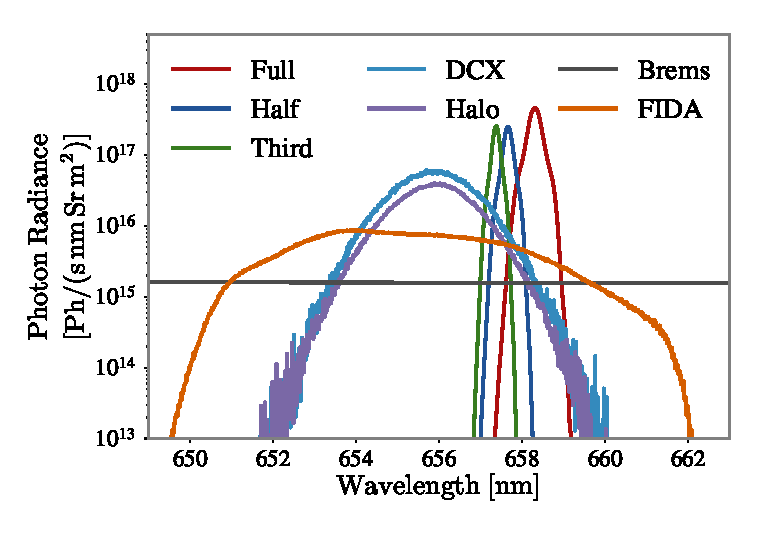
\includegraphics[width=10cm]{figures/spectra.eps}
    \caption{Spectra calculated by FIDASIM. Line of sight is viewing DIII-D 210RT neutral beam at an oblique angle in the core of the plasma.}
    \label{fig:spectra}
\end{figure}
\subsection{Spectroscopic Geometry}
Similar to the neutral beam geometry, each spectroscopic line of sight (LOS) is defined by a lens source location, an optical axis, and an optional spot size. The intersection of the LOS with the neutral beam cell is calculated using the neutral particle tracking algorithm described previously. In the original version of FIDASIM, the LOS intersections were stored in a $n_x \times n_y \times n_z \times n_{chan}$ sized grid. This caused memory issues when a large number of LOS were simulated, e.g. in a camera setup. This issue was resolved by using a sparse representation of the LOS intersections.

\subsection{Bremsstrahlung}
The largest source of background emission is visible bremsstrahlung. The local bremsstrahlung per unit wavelength is given by
\begin{equation}\label{eq:brems}
    \frac{dN_B}{d\lambda} = 7.57\times10^{-9} g\frac{n_e^2 Z_{eff}}{\lambda T_e^{1/2}}e^{-hc/\lambda T_e}\,,
\end{equation}
where $\lambda$ is the wavelength in angstroms, $n_e$ and $T_e$ is the electron density in $cm^{-3}$ and temperature in eV respectively. The gaunt factor, $g$, depends on $T_e$ and $Z_{eff}$. It can be approximated by
\begin{equation}\label{eq:gaunt}
    g = 5.542 - (3.108 - \ln(T_e/1000))(0.6905 - 0.1323/Z_{eff})\,.
\end{equation}
To calculate the total emission, the local emissivity is integrated over the line of sight.\cite{van2010imaging}

\subsection{Emission From Neutrals}
The emissions from neutrals are collected during the neutral density calculations. The photon radiance produced by a cell can be derived from Equation \ref{eq:photon_radiance} and is given by
\begin{equation}\label{eq:cell_photon_radiance}
    L_\gamma = \frac{1}{4\pi V_{cell}} L_{cell} \Phi_\gamma\,,
\end{equation}
where $V_{cell}$ and $L_{cell}$ is the volume and LOS intersection of the cell respectively, and $\Phi_\gamma$ is the photon flux given by Equation \ref{eq:photon_flux}.
The photon radiance is then distributed among the stark components in accordance with Equations \ref{eq:wavelengths} and \ref{eq:stark_intens}. Summing the spectra over the LOS cells gives the total spectra.

Calculating the neutral beam spectra during the neutral density calculation is the preferred method as it correctly models the neutral particle velocity distribution. However, in addition to the cold edge neutrals, FIDASIM offers the ability to preload the beam, DCX and halo neutral densities. In these cases, only the total photon radiance produced by a cell is known. In order to calculate the spectrum, it is assumed that the photon radiance is equally split between the neutral particles within the cell. A distribution of the neutral particle velocities within the cell is also assumed. In the case of the beam neutrals, Equation \ref{eq:beam_distribution} is used, otherwise the local ion velocity distribution is used. The spectrum is then calculated by drawing samples from the velocity distribution and averaging the resultant spectrum. The total spectra is found by summing the spectra produced over the LOS. The quality of the approximate spectrum depends on the accuracy of the underlying assumptions. Figure \ref{fig:approx_spectra} compares the approximate spectra with the full simulation.
\begin{figure}[h!]
    \centering
    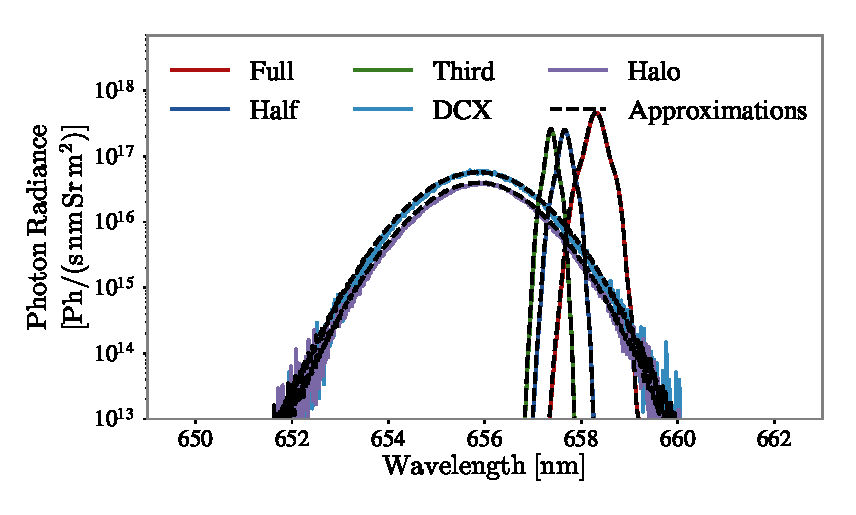
\includegraphics[width=12cm]{figures/approx_spectra.eps}
    \caption{Comparisons of full neutral beam spectra calculation (colored lines) and approximate method (black dashed overlay). The line of sight views the core region at an oblique angle.}
    \label{fig:approx_spectra}
\end{figure}

\section{Simulation of Neutral Particle Analyzers}
Neutral particle analyzers collect fast neutrals that escape the plasma. However, since most fast-neutral trajectories miss, simulating the detectors require a ridiculous number of trajectories to even have a chance of hitting the detector. Originally, FIDASIM could only use this approach, which was practically useless because of the computational cost---a single NPA simulation with good statistics could take more than a week. In the latest versions of FIDASIM, this issue has been rectified for guiding center distributions by \textit{a priori} calculating the range of trajectories that would hit the detector. This required improvements to the NPA geometry.

\subsection{NPA Geometry}
\begin{figure}[h!]
    \centering
    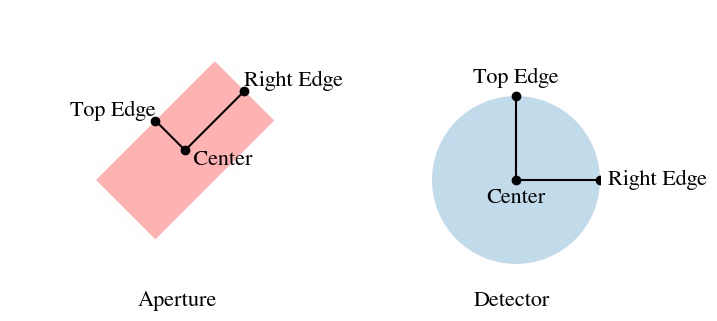
\includegraphics[width=15cm]{figures/npa_geom.jpg}
    \caption{NPA geometry definition. An aperture/detector is defined by three points, (u,v,w), which define a plane. As viewed from inside the vessel the three points are: the center, the top edge, and the right edge. The shape of the aperture/detector can either be rectangular or circular/ellipsoidal.}
    \label{fig:npa_geom}
\end{figure}
The NPA geometry in the original FIDASIM was only defined by a location, axis, and opening angle. If the entire neutral trajectory was within the cone defined by the opening angle, the neutral particle was accepted. This original definition didn't take into account the finite detector/aperture shapes and assumed rotational symmetry around the detector axis.
In newer versions of FIDASIM, the NPA geometry was changed. In the new version, the NPA detector is assumed to have an aperture and detector. Both the aperture and the detector are defined by three points which define a bounded plane: the center of the aperture/detector, the center of the top edge, and the center of the right edge. These points, along with a shape indicator, define the size of the aperture/detector as well as define a coordinate system with the +z axis normal to the plane. The apertures and detectors can be arbitrarily oriented. Figure \ref{fig:npa_geom} summarizes the NPA geometry definition.

\begin{figure}[h!]
    \centering
    \includegraphics[width=10cm]{figures/inpa.eps}
    \caption{DIII-D's imaging NPA. FIDASIM models the pinhole aperture and the stripping foil as the detector. Curved trajectories to the phosphor plate are calculated in post-processing. Image complement of Xiaodi Du.}
    \label{fig:inpa}
\end{figure}
The new NPA geometry is very flexible and can be used to describe novel NPA configurations. For instance, DIII-D's new imaging NPA (INPA)\cite{du2018inpa}, shown in Figure \ref{fig:inpa}, has a small circular pinhole aperture and a long skinny rectangular stripping foil, which is modeled as the detector.\cite{du2018inpa}

\subsection{NPA Calculation via Solid Angles}
Instead of relying on Monte Carlo trajectories to determine which fast neutrals contribute to the NPA signal, the geometric effects can be explicitly calculated\cite{stagner2014geometric}.
The geometric factor, $f_g$, of a detector is proportional to its solid angle. The geometric factor is given by
\begin{equation}
\label{eq:solid_angle}
f_g = \frac{1}{4\pi} \iint_S \frac{\mathbf{r}\cdot\hat{\mathbf{n}}\,\,dS}{r^3}\,,
\end{equation} 
where $S$ is the viewable detector area. For most cases, this equation cannot be solved analytically hence the need for Monte Carlo methods.

NPA detectors with an aligned circular aperture and detector can be described by three parameters: the aperture radius ($R_a$), the detector radius ($R_d$), and the separation between the aperture and the detector ($H$). At some positions, the aperture cuts off portions of the detector, reducing the detecting surface $S$ and complicating the solid angle calculation. Thomas \emph{et. al.} \cite{thomas1972analytical} calculated the detecting surface $S$ by projecting the ``shadow'' created by the aperture onto the detector. This ``aperture shadow'' is parametrized by the angle of incident flux $\theta$. For an isotropic distribution of incident particles, the total geometric factor of the detector is given by
\begin{equation}
\label{eq:tot_gf}
f_g= 2\pi\int_0^{\theta_{m}}S(\theta)\sin(\theta)\cos(\theta)\,d\theta\,,
\end{equation}
where $\theta_{m}$ is the maximum angle of incidence. This expression---and others like it---have been used in analyzing NPA detectors for decades. 

When simulating NPA detectors, Equation \ref{eq:tot_gf} is of limited use since it does not parametrize the aperture shadow $S$ by position. We can do this by circumscribing the aperture onto the detector plane. Defining the detector to be on the $z=0$ plane with the normal vector co-linear with the z-axis, a source at point $(x_p,y_p,z_p)$ projects a circle onto the detecting plane with radius and center given by
\begin{equation}
\label{eq:shadow_radius}
R_s = \frac{R_a z_p}{z_p - H}
\end{equation}
and
\begin{equation}
\label{eq:shadow_center}
\vec{r}_{center} = \left(\frac{H x_p}{H-z_p} , \frac{H y_p}{H-z_p} ,0\right)\,,
\end{equation} 
where $z_p > H$. Integrating over the intersection of this circle and the detector circle gives an analytic expression for the aperture shadow $S(x_p,y_p,z_p)$.

\begin{figure}[h!]
    \centering
    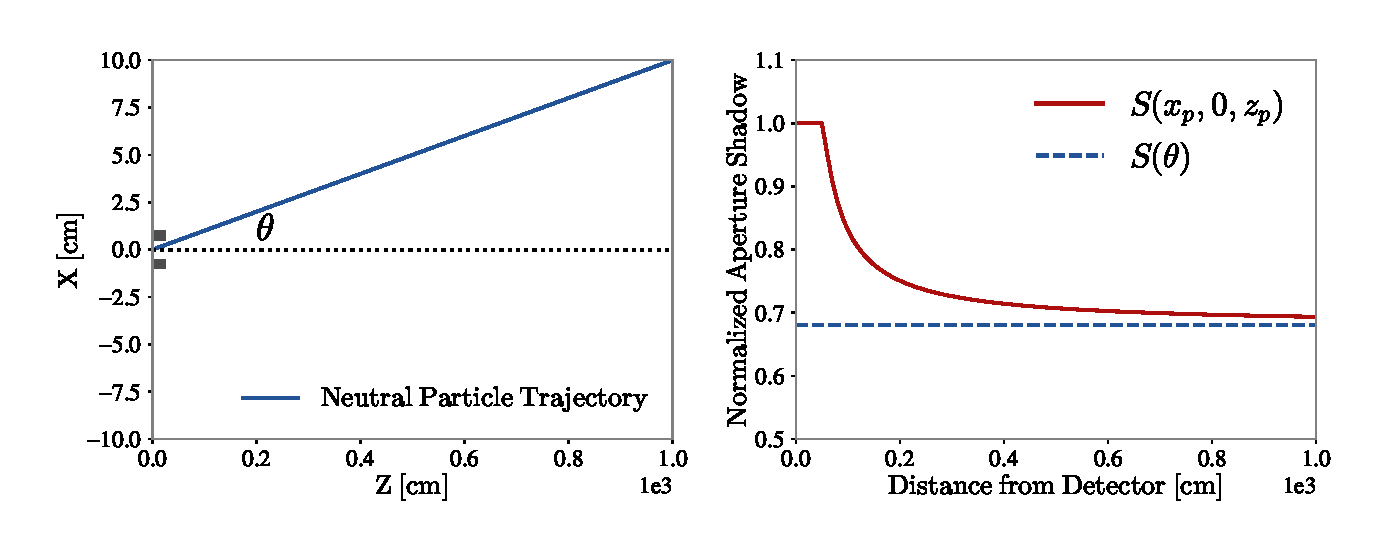
\includegraphics[width=15cm]{figures/aperture_shadow.eps}
    \caption{Left: Trajectory of a neutral particle hitting a circular NPA detector with $R_a=R_d = 0.5$ cm, and $H= 25.4$ cm. Right: Normalized aperture shadow along the particle trajectory.}
    \label{fig:shadow_compare}
\end{figure}
The two expressions for the aperture shadow ($S(\theta)$ and $S(x_p,y_p,z_p)$) should be equivalent. However, comparing the two expressions reveals a discrepancy. 
Figure \ref{fig:shadow_compare} shows that at a constant angle of incidence, the shadow area, $S(x_p,y_p,z_p)$ asymptotically approaches $S(\theta)$ as the distance from the detector increases. The discrepancy arises because $S(\theta)$ implicitly assumes that the particle source is far away from the detector (far-field assumption) and can be parameterized by a single angle of incidence. 

To understand this, consider an isotropically emitting source. Far away from the detector the choice of angle of incidence $\theta$ is trivial since they are approximately the same for every trajectory that strikes the detector. When the source is near the detector, the choice of angle of incidence is not as clear since there are many possible particle trajectories each with a significantly different angle of incidence. As the particle source moves away from the detector, the possible angles of incidence approach a single value. 
However, for NPA detectors the particle source is relatively close to the detector aperture (~0.5 m); violating the requirements needed to use the $\theta$ parametrized geometric factor. Instead, a brute force application of Equation \ref{eq:solid_angle} over the aperture shadow should be used.

As mentioned, the calculation of the solid angle can be challenging; however, there is an alternative.
The geometric factor can be thought of as the probability of a particle hitting the detector from a point $\vec{p}$ above the detector. The problem of calculating the geometric factor of the detector becomes an exercise of mapping the probability density function at the source onto the detector plane $z=0$. In general, the mapping from $\mathbf{Y}$ to $\mathbf{X}$ space is done through the change in variable equation 
\begin{equation}
\label{eq:change_of_variables}
prob(\mathbf{X}) = prob(\mathbf{Y}) \times \left | \frac{\partial \mathbf{Y}}{\partial \mathbf{X}} \right|\,,
\end{equation}
where the term on the far right is the Jacobian of the transformation.\footnote{The transformation $X = H(Y)$ is subject to the constraint that $H$ is bijective and differentiable. If $H$ is not bijective Eq. \ref {eq:change_of_variables} can be extended to a summation over all the $Y$ values that correspond to a given $X$.}

In the case of NPA detectors, the transformation is from $\{\phi,\theta\}$-space, where $\phi$ and $\theta$ are the azimuthal and polar angle respectively, to $\{x,y\}$-space. For linear trajectories, the transformation is given by
\begin{equation}
\label{eq:matrix_transform}
\begin{bmatrix}
	x \\
	y \\
	0 \\
\end{bmatrix}
=
\begin{bmatrix}
	1 & 0 & \tan{\theta}\cos(\phi)\\
	0 & 1 & \tan{\theta}\sin(\phi)\\
	0 & 0 & 0\\
\end{bmatrix}
\begin{bmatrix}
	x_p \\
	y_p \\
	z_p \\
\end{bmatrix}\,,
\end{equation}
where $(x_p,y_p,z_p)$ is the position of the particle source. The Jacobian for this transformation is given by
\begin{equation}
\label{eq:jacobian}
\left | \frac{\partial(\phi,\theta)}{\partial(x,y)} \right| = \frac{z_p ((x-x_p)^2 + (y-y_p)^2)^{-1/2}}{(x-x_p)^2 + (y-y_p)^2 + z_p^2}\,.
\end{equation}
For an isotropic source, the probability density function in $\{\phi,\theta\}$-space is given by 
\begin{equation}
\label{eq:source_pdf}
prob(\phi,\theta) = \frac{1}{4\pi} \sin(\theta)\,.
\end{equation}
Plugging equation \ref{eq:source_pdf} and \ref{eq:jacobian} into the change of variable equation and integrating over the aperture shadow $S(x_p,y_p,z_p)$ yields the geometric factor,
\begin{equation}
\label{eq:prob_geo}
f_g = \frac{1}{4\pi}\iint_S\frac{z_p\,\, dS}{((x-x_p)^2 + (y-y_p)^2 + z_p^2)^{3/2}}\,.
\end{equation}
\begin{figure}[h!]
    \centering
    \includegraphics[width=15cm]{figures/npa_prob.eps}
    \caption{Geometric Factor/Probability of hitting DIII-D's solid state NPA detector. Probability evaluated on the $y=0$ plane. Dashed lines are detecting limits.}
    \label{fig:npa_prob}
\end{figure}

For circular detectors, the detecting region can be found by using Equations \ref{eq:shadow_radius}-\ref{eq:shadow_center}; however, for arbitrarily oriented and shaped apertures/detectors the detecting region is determined by checking whether the trajectories from the source to a point on the detector passes through the aperture.
Figure \ref{fig:npa_prob} shows the geometric factors/probabilities of hitting one of DIII-D's solid state NPA detector. As can be seen, the probability is extremely small and demonstrates why the traditional method of calculating NPA signal is inefficient. 

With the probabilistic formulation, we are also able to find the average strike point on the detector. Combined with the fast-neutral starting point, we are then able to calculate the pitch, $p_t$, of the fast neutral as well as a representative trajectory from the source to the detector. With this information, we can establish the initial population flux of the fast-neutral, which is the same as Equation \ref{eq:fast_rates} with the $N_f/N_t$ term replaced with $2*F(E,p_t,R_s,Z_s)*f_g*V_{cell}*dE$; the factor of two is needed to convert the fast-ion distribution units from $N_f/(dE\,dp\,dR\,dZ)$ to $N_f/(dE\,dR\,dZ\,d\Omega/4\pi)$, i.e. to use the same units as the geometric factor. The collisional radiative model is then solved along the track and total population flux is then stored. Figure \ref{fig:npa_flux} shows the fast-neutral energy flux incident on the stripping foil for the DIII-D's INPA diagnostic. Using this approach, the computational time was drastically reduced from days to minutes.

\subsection{NPA Calculation via Gyro Angles}
While the previously discussed solid angle based NPA calculation is suitable for fast-ion distribution functions, Monte Carlo distributions require a different approach. Instead of calculating the solid angle, which is irrelevant for Monte Carlo distributions, we analytically find the range of gyro-angles that intersect the NPA detector for each MC particle. 

If we assume that the magnetic field does not change substantially over a Larmor radius, we can then take the gyro-radius to be constant, forming a ring around the particle. A neutral particle is ``fired'' from this ring at a constant pitch, $p$. If we vary the gyro-angle, $\gamma$, the surface of revolution formed by the neutral trajectory creates a ruled surface, specifically a hyperboloid of one sheet (Fig. \ref{fig:npa_intersect}). This ``gyro-surface'' has an analytic parameterization given by
\begin{equation}\label{eq:hyperboloid}
\begin{split}
    x(\gamma,t) &= \frac{||v||\sqrt{1-p^2}}{\omega_c}\left(\cos(\gamma) - t\sin(\gamma)\right) \\
    y(\gamma,t) &= \frac{||v||\sqrt{1-p^2}}{\omega_c}\left(\sin(\gamma) + t\cos(\gamma)\right) \\
    z(\gamma,t) &= \frac{||v||}{\omega_c}t\,,
\end{split}
\end{equation}
where $p$ is the pitch, $||v||$ is the speed of the neutral particle, $\omega_c$ is the ion cyclotron frequency, and the z axis is aligned with the magnetic field.

By circumscribing the edges of both the aperture and the detector, the intersection points of the edges with the gyro-surface are found. With the intersection points the range of gyro-angles, $\Delta \gamma$, that both hit the detector and pass through the aperture can be calculated. Figure \ref{fig:npa_intersect} shows an example gyro-range for a small circular aperture and a larger circular detector.
\begin{figure}[h!]
    \centering
    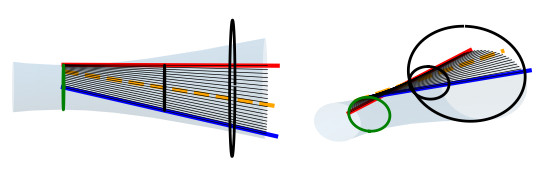
\includegraphics[width=12cm]{figures/npa_intersection.jpg}
    \caption{Two views of a (exaggerated) Gyro-surface (light blue) created by fast-neutral trajectories. The two black rings are the aperture (smaller circle) and the detector (larger circle). The green circle is the gyro-ring. The red/blue lines shows the first/last trajectory to pass through the aperture and hit the detector. The dashed orange line shows the representative trajectory used for the collisional radiative model. The thin black lines shows the trajectories over which the neutral flux is distributed.}
    \label{fig:npa_intersect}
\end{figure}

The initial population flux is the same as Equation \ref{eq:fast_rates} with the $N_f/N_t$ term replaced with $w_i\Delta\gamma/2\pi$. Since the path length of the trajectories within the gyro-range are similar, the collisional radiative model is only calculated for the middle trajectory. The neutral flux is then equally distributed among the other trajectories in the range. This is done so that the particles that hit the detector are not biased towards the center of the detector. This approach also drastically sped up the NPA calculation and is now comparable to the FIDA calculation. It is also equivalent with the previously discussed method. Figure \ref{fig:npa_flux} compares the solid angle approach with the gyro-angle approach. Both methods give the same neutral flux.
\begin{figure}[h!]
    \centering
    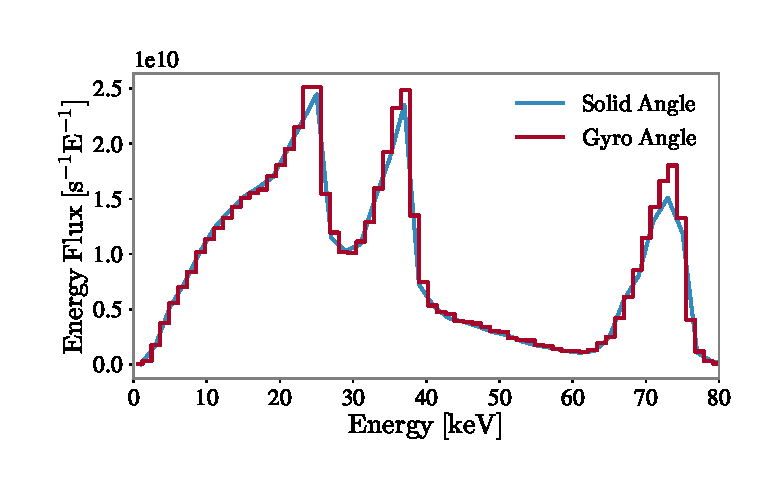
\includegraphics[width=13cm]{figures/inpa_flux.eps}
    \caption{Incident energy flux for imaging NPA: Solid angle NPA calculation (blue) and the Gyro Angle approach (red step). Both methods give the same energy flux.}
    \label{fig:npa_flux}
\end{figure}

\section{Simulation of Beam-Plasma Neutron Rates}
A recent addition to FIDASIM is the ability to calculate volume-averaged beam-plasma neutron rates. Because there are no geometric effects to consider, the calculation of the neutron rate is straight forward and is given by
\begin{equation}\label{eq:neutron_rate_f}
    \rm{rate} = \iiiint F(E,p,R,Z) \int_0^{2\pi} S_{neutron}(E,p,R,Z,\gamma) \,d\gamma\,dE\,dp\,dR\,dZ\,,
\end{equation}
where $S_{neutron}$ is the forward model of the neutron detector specified in Equation \ref{eq:W_neutron} and $F(E,p,R,Z)$ is the guiding center fast-ion distribution function.
If a guiding center Monte Carlo distribution was used, the neutron rate would be given by
\begin{equation}\label{eq:neutron_rate_gcmc}
    \rm{rate} = \sum_i^{N_p}\left (\frac{w_i}{2\pi} \int_0^{2\pi}  S_{neutron}(E_i,p_i,R_i,Z_i,\gamma) \,d\gamma \right )\,,
\end{equation}
where $w_i$ is the weight of the Monte Carlo particle such that the total number of fast ions is given by $\sum_i^{N_p} w_i$. If a full orbit Monte Carlo distribution is used, the neutron rate is given simply by
\begin{equation}\label{eq:neutron_rate_fomc}
    \rm{rate} = \sum_i^{N_p}\left (w_i S_{neutron}({v_r}_i,{v_\phi}_i,{v_z}_i,R_i,Z_i,\phi_i) \right ).
\end{equation}
From the above equations, it is plain to see that the neutron rate is just the sum of the rates from the individual fast-ions. In the next chapter, we will see that all the discussed diagnostics can be expressed in a similar manner.